\section{SDSS and MaNGA data}
Small intro related to galaxies: \\
Galaxies in a nutshell:\\

\begin{itemize}
  \item ''$\Lambda$CDM tells us that dark matter halos grow from the 'bottom up', hierarchically assembling into increasingly massive structures with time'' \citep{bundy2015}
  \item ''The fundamental components of present-day galaxies formed as a result of various complex processes that act on the baryons residing in these evolving halos'' \citep{bundy2015}
\end{itemize}

SDSS and MaNGA have and will help us understand the physics of galaxies as well as the mechanisms that drive their evolution.

\subsection{Sloan Digital Sky Survey (SDSS)}

\subsubsection*{SDSS Scientific Motivation}

\subsubsection*{SDSS Survey Design}

\subsubsection*{SDSS Data Components and Metadata}

\subsubsection*{SDSS Data Curation}

%%%%%%%%%%%%%%%%%%%%%%%%%%%%%%%%%%%%%%%%%%%%%%%%%%%%%%%%%%%%%%%%%%%%%%%%%%%%%%%%%%%%%%%%%%%%%%%%%%%%%%%%%%%%%%%
\subsection{Mapping Nearby Galaxies at APO: MaNGA}

MaNGA is a survey component from the Sloan Digital Sky Survey (SDSS) \citep{bundy2015, ahumada2020}. Its mission is to observe with Integral Field Units (IFUs) approximately 10.000 nearby galaxies. Thanks to the IFUs, MaNGA is able to measure the spectra of different regions of the same galaxy, depending on the number of fibers in the IFU.

\subsubsection*{MaNGA Scientific Motivation}

MaNGA is helping us to understand the physics of the mechanisms that drive the evolution of galaxies by:

\begin{itemize}

  \item Trying to understand the present growing process of a galactic disk:

  \begin{itemize}
    \item What fuels this process?
  \end{itemize}

  \item Trying to understand how stellar accretion, mergers, and secular evolution influence the growth of bulges and ellipticals.

  \item Trying to understand the influence of internal and external processes in the shutdown of star formation.
  
  \item Trying to probe the distribution of mass and angular momentum among different components.
\end{itemize}

\textbf{REFRAME IT to fii natural in this section:} As mentioned previously, the MaNGA sample size is $\sim 10.000$ galaxies. The natural question to ask is: why is this a good number for the science intended to do? A simple estimation can help us understand that:

The approximate number of bins needed per axis in the parameter space that defines a galaxy population is $\sim 6$. These axes are Stellar-mass, SFR (or morphology), and environment. The number of galaxies required per bin, satisfying the condition that the precision of a measurement is approximately equal to the expected variation of it among the bins, is $\sim 50$. This gives a rough approximation of $50 \times 63 = 10,800$ galaxies

With this sample size, MaNGA is expected to explore new regions of the parameter's space of galaxy populations. \textbf{Meaning there is an open window for new discoveries!}


\subsubsection*{MaNGA Survey Design}

 MaNGA uses the two Baryon Oscillation Spectroscopic Survey (BOSS) spectrographs, covering a wavelength range from 360 nm to 1040 nm with a resolving power of $\sim 2000$. MaNGA has a configuration that allows for the observation of 17 galaxies at a time. Each fiber used in MaNGA has a diameter of 120 microns, equivalent to 2'' and they are packed in ferrules forming a hexagonally shaped IFU, as shown in Fig. 1 below [put figure obviously].

The number of IFUs used for galaxies are 2x19, 4x37, 4x61, 2x91, and 5x127. For instance, 4x61 means that there are 4 IFUs packed in a bundle of 61 fibers. Besides 12x7 IFUs are used for calibration and 92 fibers are used to sample the sky near each target galaxy, this for a total of 1423 fibers. 

\begin{enumerate}
  
  \item The fiber diameter is of $\sim 2''$, matched to a typical ground-based seeing.
  
  \item S/N requirement in the outskirts: $5-10$ \AA$^{-1}$
  
  \item The outskirts of the target are assumed to be located at $1-2$ $R_e$
  
  \item Required exposure time: $\sim 3$ $hr$

  \item To reach a physical scale of $\delta =$ $1$ $kpc$ with a $2''$ fiber diameter, it demands a $z \sim  0.03$
  
  \item Volumetric density of galaxies with $M > 109 M_{\odot}$ $+$ observing area of $\sim 3500$ $deg^2 \rightarrow z > 0.03$  , in order to obtain  $\sim 10.000$ galaxies.
  
  \item The number of fibers used is 1423
  
  \item Fiber budget + IFUs size + dynamic range of $R_e \rightarrow 0.03 < z < 0.10$
  
  \item It translates in targeting larger galaxies at greater distances.
  
  \item $ \sim 20$ IFUs ($3°$ FoV) + $3$ hr exposure + $ \sim 500$ plates $\rightarrow 190$ nights.
  
  \item Accounting for weather and dark time limitations, plus time shared with eBOSS, the survey has a duration of 6 yr
\end{enumerate}

In regard to the fibers and the fiber bundles, we have:

\begin{enumerate}
  \item The number of fibers used is $1423$
  
  \item Each fiber has a $2''$ diameter on-sky.
  
  \item The IFUs are $19$ to $127$ fibers in size, packed in an hexagonal shape. 
  
  \item The diameters range is from $12''$ to $32''$ on-sky. 
  
  \item Fibers are inserted by hand in metal ferrules. 
  
  \item The IFUs used for galaxies: $2 \times 19$; $4 \times 37$; $4 \times 61$; $2 \times 91$ ; $5 \times 127$, (1247)
  
  \item $12$ IFUs packed in bundles of $7$ are used for calibration. 
  
  \item The remaining $92$ fibers are used to sample the sky near each target
  
  \item The IFUs have a fill factor of $ \sim 56 \%$. 
  
  \item The cross-talk between spectral traces of adjacent fibers is of $ \sim 10 \%$
\end{enumerate}

\subsubsection*{Data Components and Metadata}

The MaNGA Data Reduction Pipeline (DRP) \citep{law2016} takes the raw MaNGA data and generates a data-cube, a three-dimensional data array containing spectra for a single galaxy. The array has two spatial dimensions and a wavelength dimension representing the spectra of a galaxy at each of its spatial measured points. The DRP generates the DRPall summary fits file containing the metadata for all the observations, galaxies, and non-galaxies. In the case of galaxies, it includes information such as the redshift, among others drawn from the NASA-Sloan Atlas. The DAP processes only the log-linearly binned data cubes (LOGCUBE files) from the DRP to produce stellar and ionized gas kinematics, among others, stored in the MAPS files. Each MaNGA observation is uniquely identified with the plate-IFUdesing, which allows us to find a specific galaxy observation. There is also the MaNGA-ID which uniquely identifies a galaxy, this is something to have in mind since a galaxy might have multiple observations, having, therefore, several plate-IFUdesigns

MaNGA data processing needs are not a trivial task, for instance, we can plot some numbers. The sample size is of $ \sim 10,000$ low redshift galaxies, out of wich there are approximately 100 million raw-frame spectra which after reduction, go down to about 10 million reduced spectra.
The processing of the raw data has to take into account many variables related to the exposition time, too.

The MaNGA Data Reduction Pipeline (DRP) is aimed at producing a flux calibrated spectral cube of galaxies in a FITS format. The DRP is written mainly in IDL, aided by C and python scripts. The DRP consists of two stages:

\begin{enumerate}
  \item 2d stage: flux-calibrated fiber spectra
  
  \item 3d stage: products from 2D stage + astrometric information $\rightarrow$ data cubes
\end{enumerate}

For the 2d stage the product consists of flux-calibrated individual exposures of an entire plate, that is, the science and calibration exposures.All the calibrations exposures are processed to determine the spatial trace of the fiber on the detector in order to extract fiber flat-field and wavelength calibration vectors. The products above are used to process science frames. From the sky fibers a super-sampled model of the sky background is created to then be subtracted from each fiber spectra. The mini-bundles used for standard stars are used to determine the flux calibration vector for the exposure. The final product is a 2D FITS file with Row-Stacked Spectra (RSS), ie, each row is the spectra of each of the 1423 fibers.  
 
For the 3d stage The products consist of data cubes and RSS for a galaxy from all the exposures. Once the needed number of exposures is completed per plate, the 3d stage is triggered using all the RSS FITS files generated in the 2d stage. The RSS FITS files of a plate are combined in this stage. The relevant spectra of a target for the exposures are identified and sorted using astrometric information. A data cube is generated for each target, having additional products: griz image, mask cube, reference information and more. The final products of the 3d stage are used later with the Data Analysis Pipeline (DAP) built for MaNGA to produce science data products.

Given the complexity of all the data processing stage, it is good to keep in mind that in addition to what was mentioned above different operational variables change and in different time scales, therefore the need for metadata track, eg: fiber bundle metrology, cartridge layout, fiber plugin locations and more. Metadata is essential if we want to rerun the DRP to obtain data products.

\begin{figure}[h!]
  \centering
    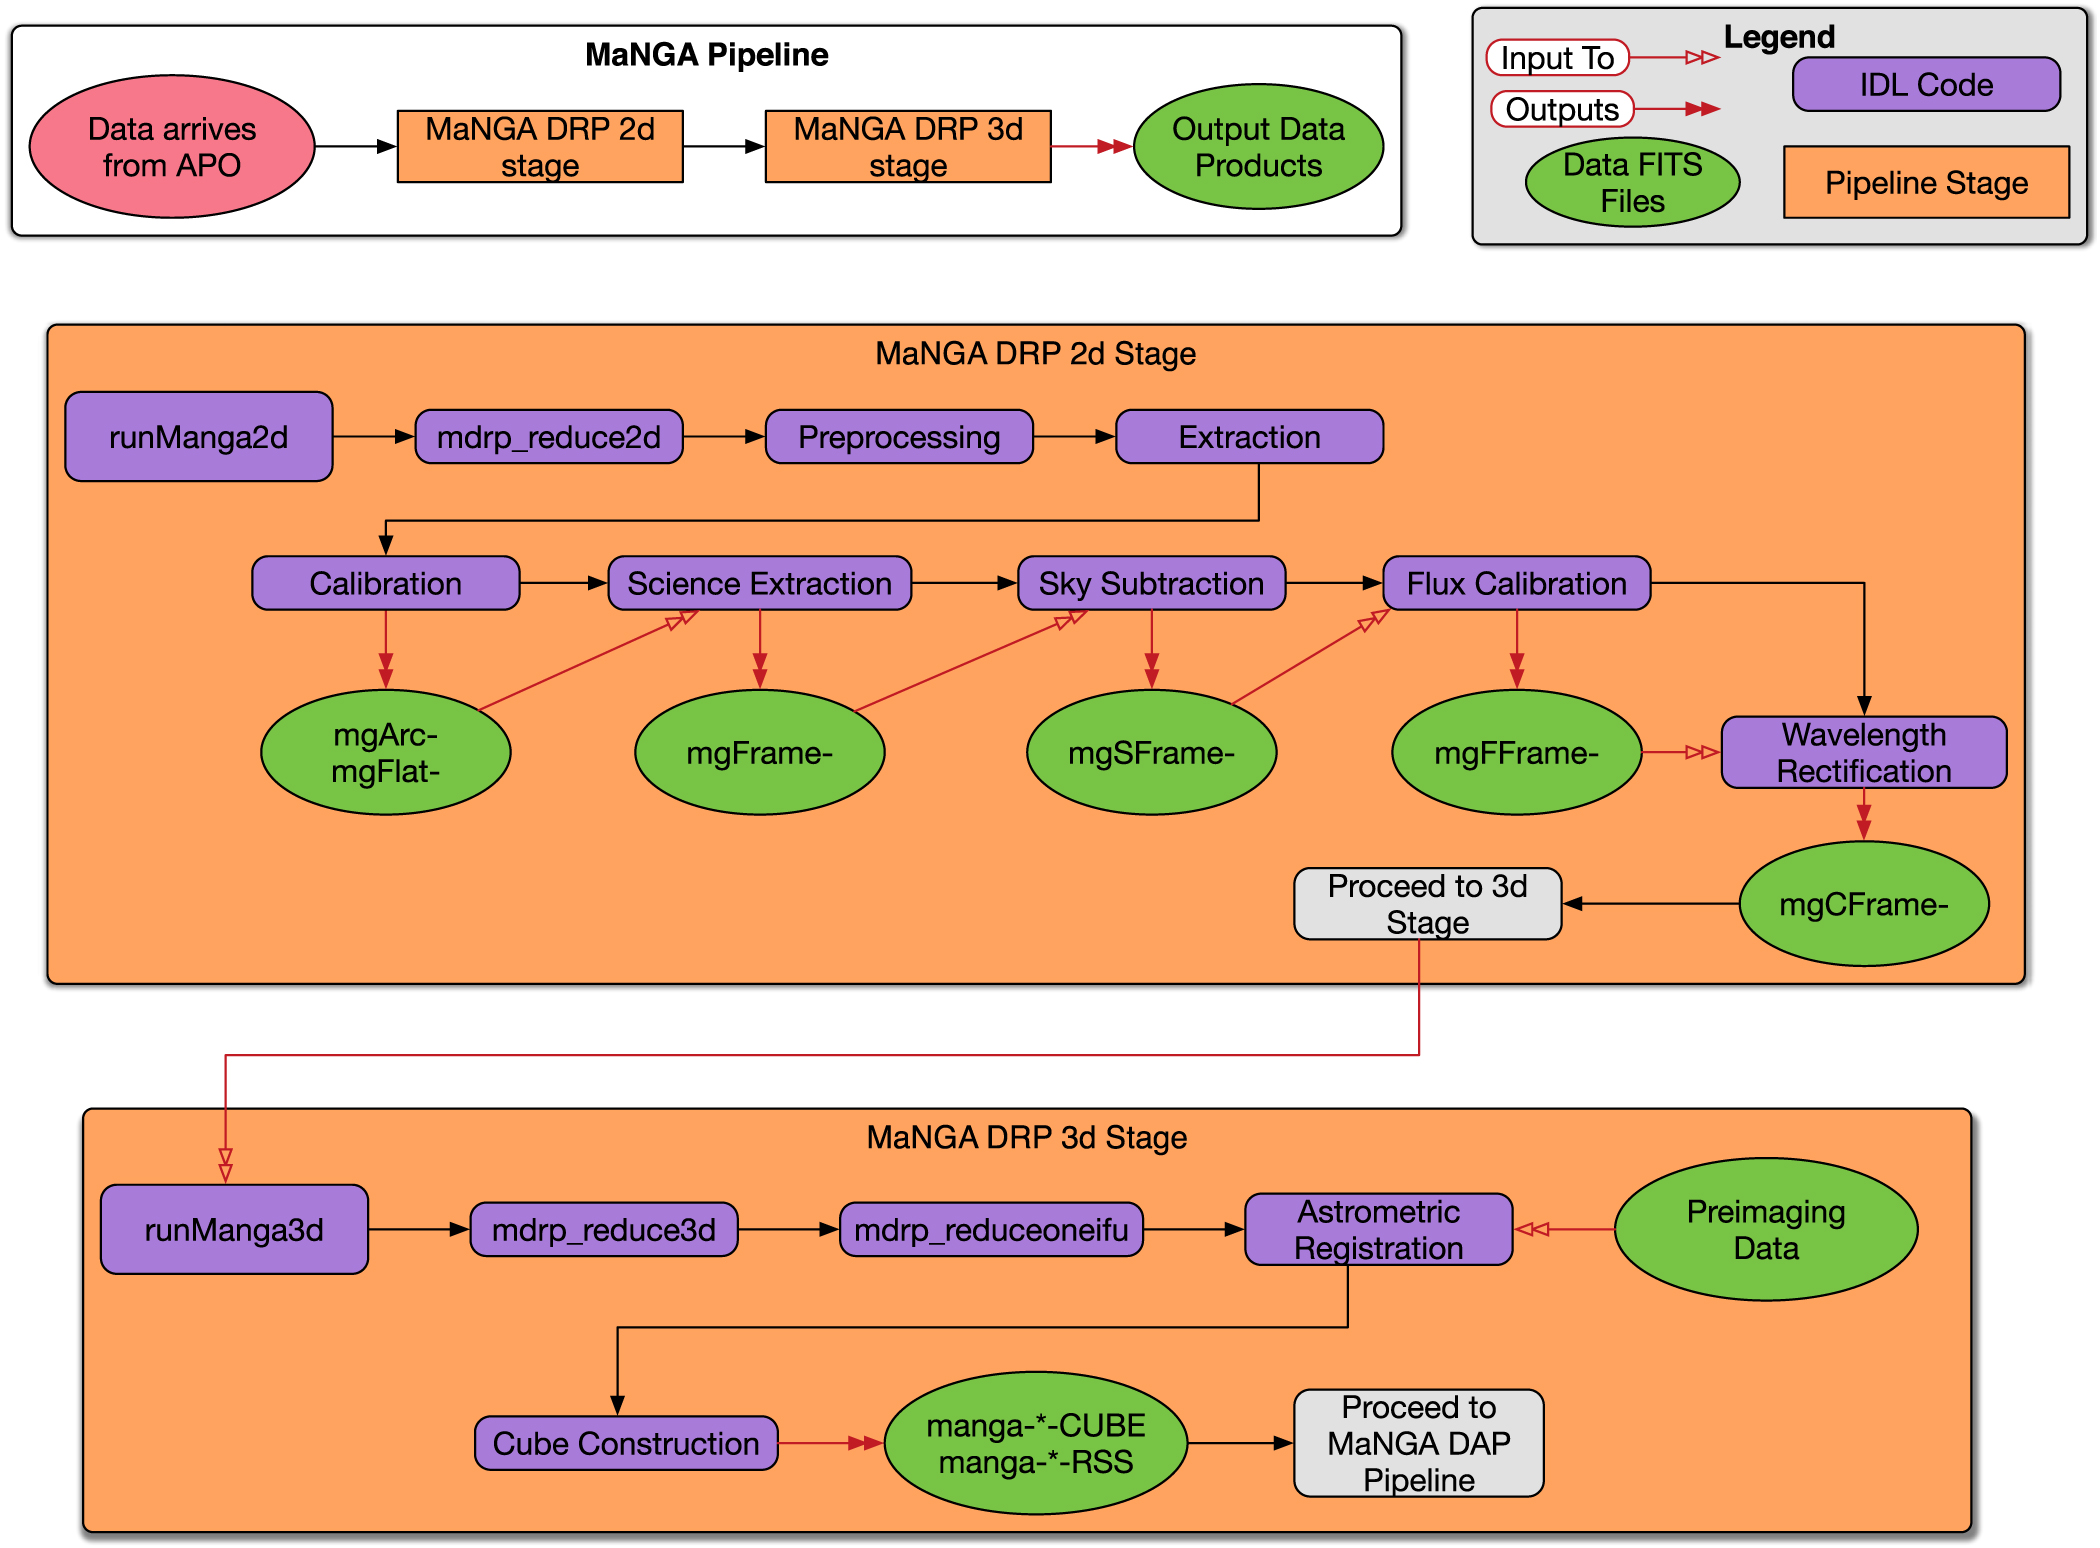
\includegraphics[width=0.9\textwidth]{MaNGA_DRP_diagram.jpg}
  \caption{\small{MaNGA DRP diagram \citep{law2016}}}
  \label{fig: outlier_URF}
\end{figure}

\subsubsection*{MaNGA Data Curation}

ML algorithms are agnostic in the sense that they don't know what is the phenomenology behind the data used for their training. For instance, let's assume we have the same spectrum of a galaxy but with different redshifts. If we feed these spectra to the ML algorithm, it is going to think that we have two different objects. Therefore before developing an ML model it is necessary to correct for these kinds of situations in order to make comparisons meaningful. Additionally, we can not just feed raw data to the algorithm because there are scenarios where we have missing values, artifacts. MaNGA data provides several flags signaling scenarios of these kinds for the data. Table \ref{table:MaNGA Data Quality Mask Bits} provides these values:

\begin{table}[h!]
\centering
\begin{tabular}{|c|c|l|} 
 \hline
 Key & Bit & Description \\ [0.5ex] 
 \hline
 FORESTAR & 0 & There is a FORESTAR region within the data cube \\ 
 \hline
 BADZ & 1 & NSA redshift does not match derived redshift (placeholder) \\
 \hline
 LINELESS & 2 & No emission lines in data cube (placeholder) \\
 \hline
 PPXFFAIL & 3 & pPXF failed to fit this object (placeholder) \\
 \hline
 SINGLEBIN & 4 & Voronoi binning resulted in all spectra in a single bin \\
 \hline
 BADGEOM & 5 & Invalid input geometry; elliptical coordinates and effective radius are meaningless. \\
 \hline
 DRPCRIT & 28 & A critical failure in DRP \\
 \hline
 DAPCRIT & 29 & A critical failure in DAP \\ 
 \hline
 CRITICAL & 30 & A critical failure in DRP or DAP \\ [1ex] 
 \hline
\end{tabular}
\caption{MaNGA Data Quality Mask Bits}
\label{table:MaNGA Data Quality Mask Bits}
\end{table}

During the data curation process, all MaNGA data with any of the mask-bits listed in Table 1 were ignored.

Some data products are two-dimensional maps of:

\begin{enumerate}
  \item  stellar velocity and velocity dispersion, 
  
  \item mean stellar age and star formation history, 
  
  \item stellar metallicity, 
  
  \item element abundance ratio, 
  
  \item stellar mass surface density, 
  
  \item ionized gas velocity, 
  
  \item ionized gas metallicity, 
  
  \item star formation rate and 
  
  \item dust extinction
\end{enumerate}
